
\documentclass[reprint,amsmath,aps,nofootinbib,english]{revtex4-2}

\usepackage{graphicx}
\usepackage{dcolumn}
\usepackage{url}
\usepackage{siunitx}
\usepackage{float}

\AtBeginDocument{\renewcommand{\natexlab}[1]{#1}}% <--- the fix
\begin{document}

\title{Radioactive Decay}
\author{Tan Aytekin}
\email[]{tan.aytekin@boun.edu.tr}
\affiliation{Physics Department, Bogazici University, Istanbul, Turkey}
\collaboration{Partner : Özgür Aydın}
\date{\today}


\begin{abstract}
In this experiment, we tried to observe phenomenon called radioactive-decay by applying high-voltage to radioactive nuclei. Using the relationship between amount of decay and current, we found half-time for $^{232}Th$ isotope as  $t_{1/2} = (58.1 \pm 0.2) s$. The result is too much sigmas away(about $12 \sigma$'s) from accepted value $55.6 s$. However, because of the relative uncertainty and percentage error is low and taking into account the possible errors, it can be considered as a not bad result. 


\end{abstract}

\maketitle

\section{Introduction}
An unstable nucleus does not have enough binding energy to hold the nucleus together for a long time. Eventually, to be stable, it releases energy and matter by transmuting to another nucleus. \cite{int1} This process is called radioactive decay and it usually occurs with chain reactions. In these reactions, it releases various particles like alpha, beta, gamma particles or neutrons, etc.\cite{int2} In our experiment, we tried to study the one-decay process which is decaying of a nucleus to another nucleus only.\cite{int3} The other chain reactions are ignored.


\subsection{History}
Radioactivity was first discovered in 1896, by the French scientist Henri Becquerel while he was working on phosphorescent materials to study x-rays which discovered the previous year by Wilhelm Röntgen.\cite{hist1} After about 5 years, Ernest Rutherford and his student Frederick Soddy were discovered nuclear transmutation. They observed the radioactive thorium was converting itself into radium.\cite{hist2} Later, Marie and Pierre Curie discovered radium and polium and defined the term "radioactivity".\cite{hist3}



\section{Theory}
Universal law of radioactive decay states that decaying process of a nucleus per unit time is constant and independent of time which gives this relation:
\begin{align}
  -\frac{dN}{N} = \lambda dt
\end{align}
where $N$ is isotope unstable nuclei and $\lambda$ is decay constant. The solution of this differential equation is given by:
\begin{align}
  N(t) = N_0e^{-\lambda t} \label{eq:uni}
\end{align}
where $N_0$ is initial amount of unstable nuclei. Half-life($t_{1/2}$) which is required time for reducing initial unstable nuclei to half of its initial value can be easily calculated:
\begin{align}
  \frac{1}{2} N_0 &= N_0 e^{-\lambda t_{1/2}}\\
  t_{1/2} &= \frac{ln(2)}{\lambda} \label{eq:half}
\end{align}

Radioactive decay can be observed with various methods. One of them is to study the ionizing capability of the charged particles produced in the decay. If we apply a high voltage to a sample of radioactive nuclei, the decaying process ionizes the air which allows to flow current in the circuit. This shows that current is proportional to the amount of decay as a function of time. However, the produced current in the circuit will be too low and hard to measure. Instead of measuring the current we can measure discharge time if the amount of the maximum charge is fixed in the device: 
\begin{align}
  Q &= Is\\
  I &= \frac{Q}{s}\\
  I &\propto \frac{1}{s}\\
  \frac{1}{s(t)} &\propto N(t)\label{eq:pro}
\end{align}
where $Q$ is fixed maximum charge and $s$ is the time elapsed to reach full charge. Using \eqref{eq:uni} and \eqref{eq:pro} we get:
\begin{align}
  \frac{1}{s(t)} &= \frac{1}{s_0} e^{-\lambda t}\\
  ln\left(\frac{1}{s(t)}\right) &= ln\left(\frac{1}{s_0}\right) -\lambda t \label{eq:lneq}
\end{align}
If we measure time required to charge $s$ and plot them versus time and applying linear regression, slope of the fit gives us $-\lambda$. Later, with using \eqref{eq:half} we can find the half-time of the radioactive material in the setup.










\section{Experiment}
\subsection{Apparatus and Setup}
Our setup consists thorium salt($^{232}Th$) as a radioactive material, high-voltage power supply(0,5)kV, an ionization chamber, a stopwatch and a Wulf's electroscope which automatically discharges in a fixed charged state via connecting one of the electrodes to the ground.
\begin{figure}[H]
  \includegraphics[width=0.75\columnwidth]{graphics/app.png}
  \caption{A general schematic of the setup: High voltage applied to radioctive material in the chamber. When it is charged to maximum value Wulf's electroscope automatically discharges via grounded electrode. \cite{Gulmez}}
   \label{fig:app}
\end{figure}
When high voltage is applied to the thorium salt, radioactive decay chain occurs. The Radon gas($^{220}Rn$) is one these produced unstable nuclei that ionizes the air among the other products. Thus, in this experiment 
the decay of Radon gas studied.
\subsection{Procedure}
First, high voltage about 3-4 kV applied without adding thorium salt into the chamber to ensure there are not radioactive material left in the chamber. After making sure that there is no movement in the electroscope, high voltage is set to 2500V and then opened the clamp shutting the air flow between the thorium and ionization chamber. The bottle contains thorium salt is quickly squeezed 5 times and immediately started the timer. Time is recorded at each instant the electroscopes discharges. This process repeated 5 times for 5-7-9-11 squeezes. Later all of these steps repeated with 3.0 kV and 3.5 kV high voltage too.\\

In all measurements we accept  $\sigma_{systematic}$ as 0.2 seconds since it is the average visual response time of humans \cite{Jain2015} and $\sigma_{instrumental}$ as 0.01 seconds. Then total uncertainty is calculated with \eqref{eq:unc}. All measurements can be found in AppendixB.

\section{Data Analysis}
First, charging duration and corresponding average time calculated for all 12 sets:
\begin{align}
  s_i &= t_{i+1} - t_i \\
  T_i &= \frac{t_{i+1} + t_i}{2}
\end{align}

where $s_i$ is charging time of ith data, $T_i$ is average charging time of $t_i$ and $t_{i+1}$ where $t_i$ is the time elapsed when a discharge observed.\\

Let's plot one set of $1/s_i$ versus $T_i$:

\begin{figure}[H]
  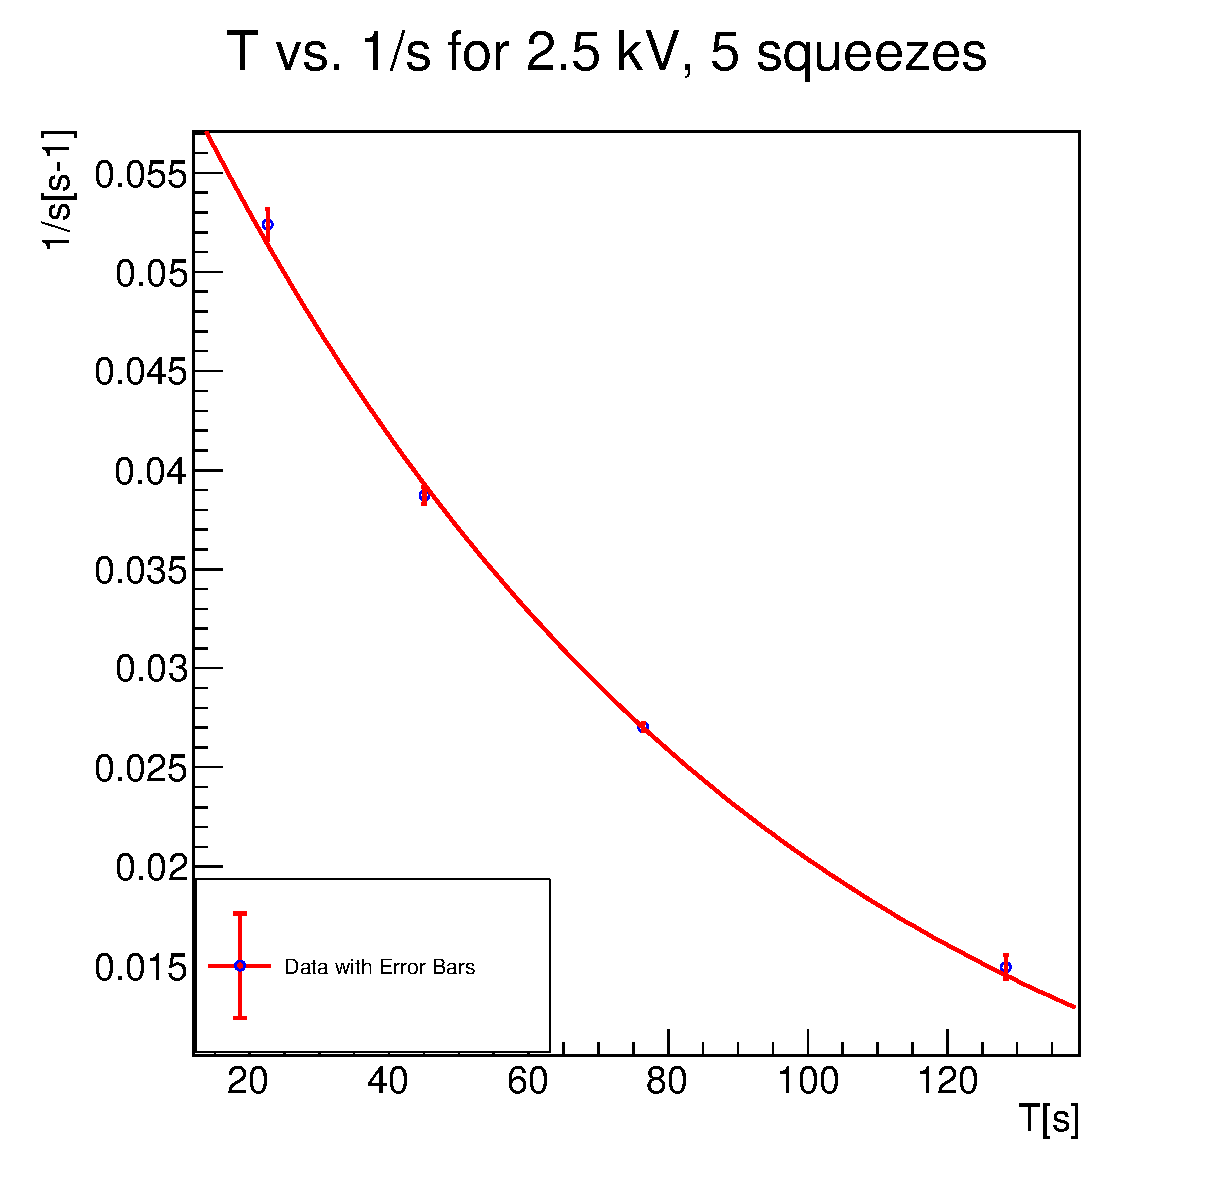
\includegraphics[width=0.95\columnwidth]{graphics/25_5T.eps}
  \caption{T vs 1/s for 2.5 kV, 5 squeezes. Exponential fit applied to show it has exponential decay since hard to see with 4 data points.}
\end{figure}

Then, $ln\left(\frac{1}{s(t)}\right)$ calculated for all datasets and plotted $T_i$ vs. $ln\left(\frac{1}{s(t)}\right)$. Linear regression applied to graphs in order to find decaying constant $\lambda$. In every calculation, error propagation \eqref{eq:err} is taken into account:

\newpage
\subsection*{2.5 kV}

\begin{table}[H]
\caption{\label{tab:k}%
Calculations for $2500\si{\volt}$ with 5 squeezes.
}
\begin{ruledtabular}
\begin{tabular}{cccc}
\textrm{T[\si{\second}]}&
\textrm{$ln\left(\frac{1}{s}\right)$} &
\textrm{$\sigma_T$[\si{\second}]} &
\textrm{$\sigma_{ln\left(\frac{1}{s}\right)}$} \\ 
\colrule  
22.57 &  -2.949 &  0.14  &   0.015 \\  
45.02 &  -3.251 &  0.14  &   0.011 \\
76.42 &  -3.611 &  0.14  &   0.008 \\
128.4 &  -4.204 &  0.14  &   0.004
\end{tabular}  
\end{ruledtabular}
\end{table}

\begin{table}[H]
\caption{\label{tab:k}%
Calculations for $2500\si{\volt}$ with 7 squeezes.
}
\begin{ruledtabular}
\begin{tabular}{cccc}
\textrm{T[\si{\second}]}&
\textrm{$ln\left(\frac{1}{s}\right)$} &
\textrm{$\sigma_T$[\si{\second}]} &
\textrm{$\sigma_{ln\left(\frac{1}{s}\right)}$} \\ 
\colrule  
13.88 & -2.608 &  0.14  &   0.021 \\   
30.54 & -2.983 &  0.14  &   0.014 \\
52.84 & -3.213 &  0.14  &   0.011 \\
86.06 & -3.728 &  0.14  &   0.007
\end{tabular}  
\end{ruledtabular}
\end{table}

\begin{table}[H]
\caption{\label{tab:k}%
Calculations for $2500\si{\volt}$ with 9 squeezes.
}
\begin{ruledtabular}
\begin{tabular}{cccc}
\textrm{T[\si{\second}]}&
\textrm{$ln\left(\frac{1}{s}\right)$} &
\textrm{$\sigma_T$[\si{\second}]} &
\textrm{$\sigma_{ln\left(\frac{1}{s}\right)}$} \\ 
\colrule  
23.29 & -2.728 &  0.14  &   0.018  \\ 
41.14 & -3.015 &  0.14  &   0.014  \\
64.40 & -3.263 &  0.14  &   0.011  \\
96.58 & -3.644 &  0.14  &   0.007
\end{tabular}  
\end{ruledtabular}
\end{table}

\begin{table}[H]
\caption{\label{tab:k}%
Calculations for $2500\si{\volt}$ with 11 squeezes.
}
\begin{ruledtabular}
\begin{tabular}{cccc}
\textrm{T[\si{\second}]}&
\textrm{$ln\left(\frac{1}{s}\right)$} &
\textrm{$\sigma_T$[\si{\second}]} &
\textrm{$\sigma_{ln\left(\frac{1}{s}\right)}$} \\ 
\colrule  
24.10  & -2.837 &  0.14  &   0.016 \\  
42.78  & -3.009 &  0.14  &   0.014 \\
67.40  & -3.367 &  0.14  &   0.010 \\
104.36 & -3.805 &  0.14  &   0.006
\end{tabular}  
\end{ruledtabular}
\end{table}

\begin{figure}[H]
  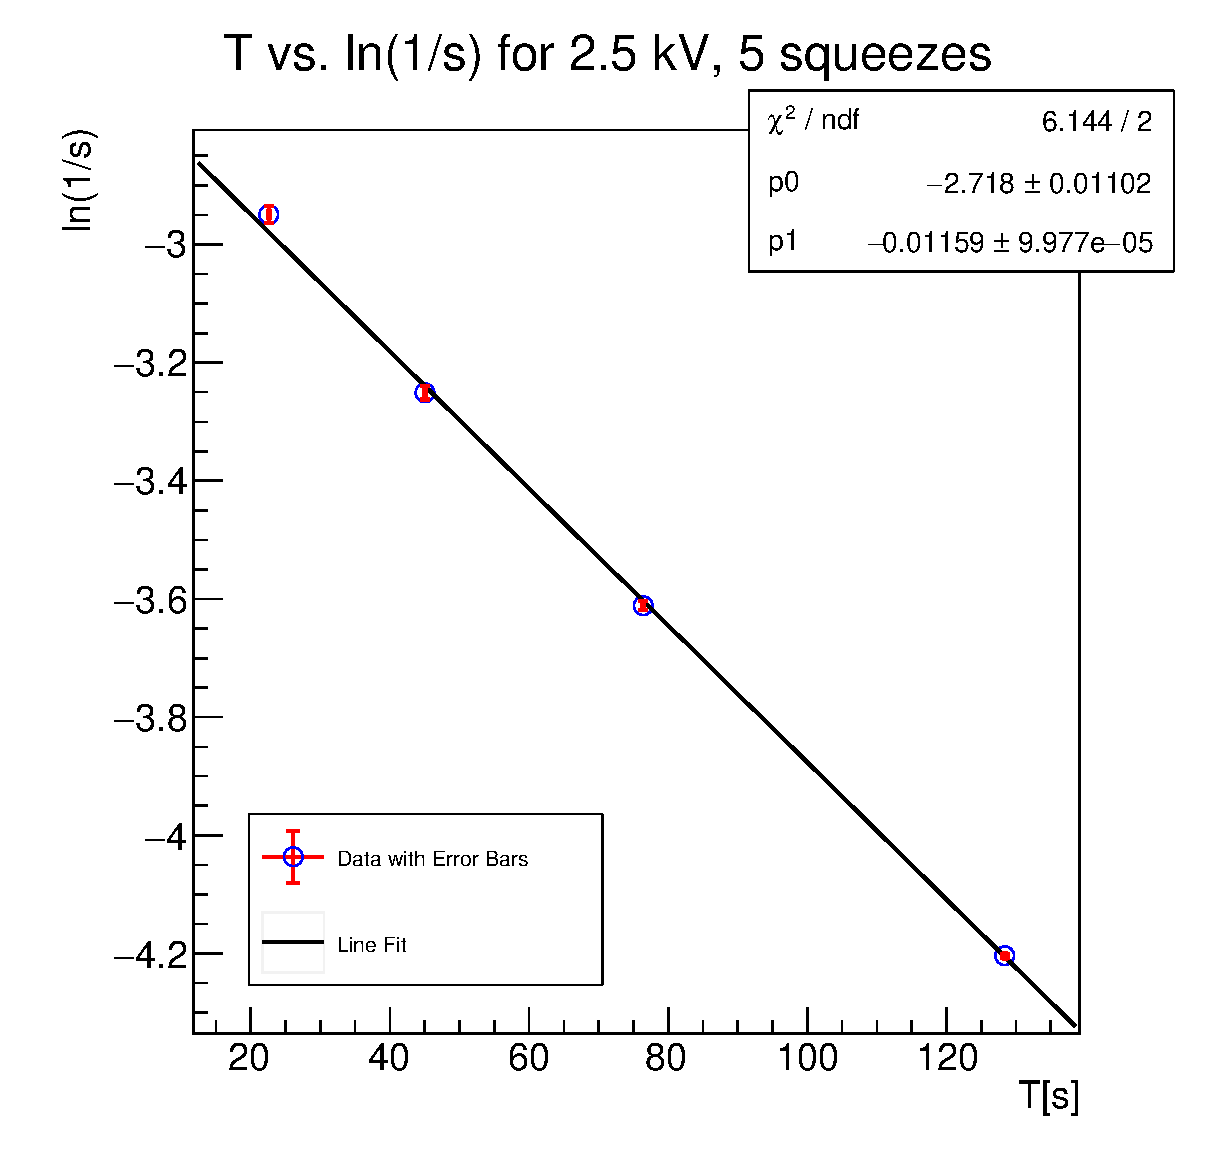
\includegraphics[width=0.95\columnwidth]{graphics/25_5.eps}
  \caption{Line regression for 2.5 kV and 5 squeezes. At each data point, error bars are drawn, where p0 is the y-intercept and p1 is the slope.}
\end{figure}




\begin{figure}[H]
  \includegraphics[width=0.95\columnwidth]{graphics/25_7.eps}
  \caption{Line regression for 2.5 kV and 7 squeezes. At each data point, error bars are drawn, where p0 is the y-intercept and p1 is the slope.}
\end{figure}




\begin{figure}[H]
  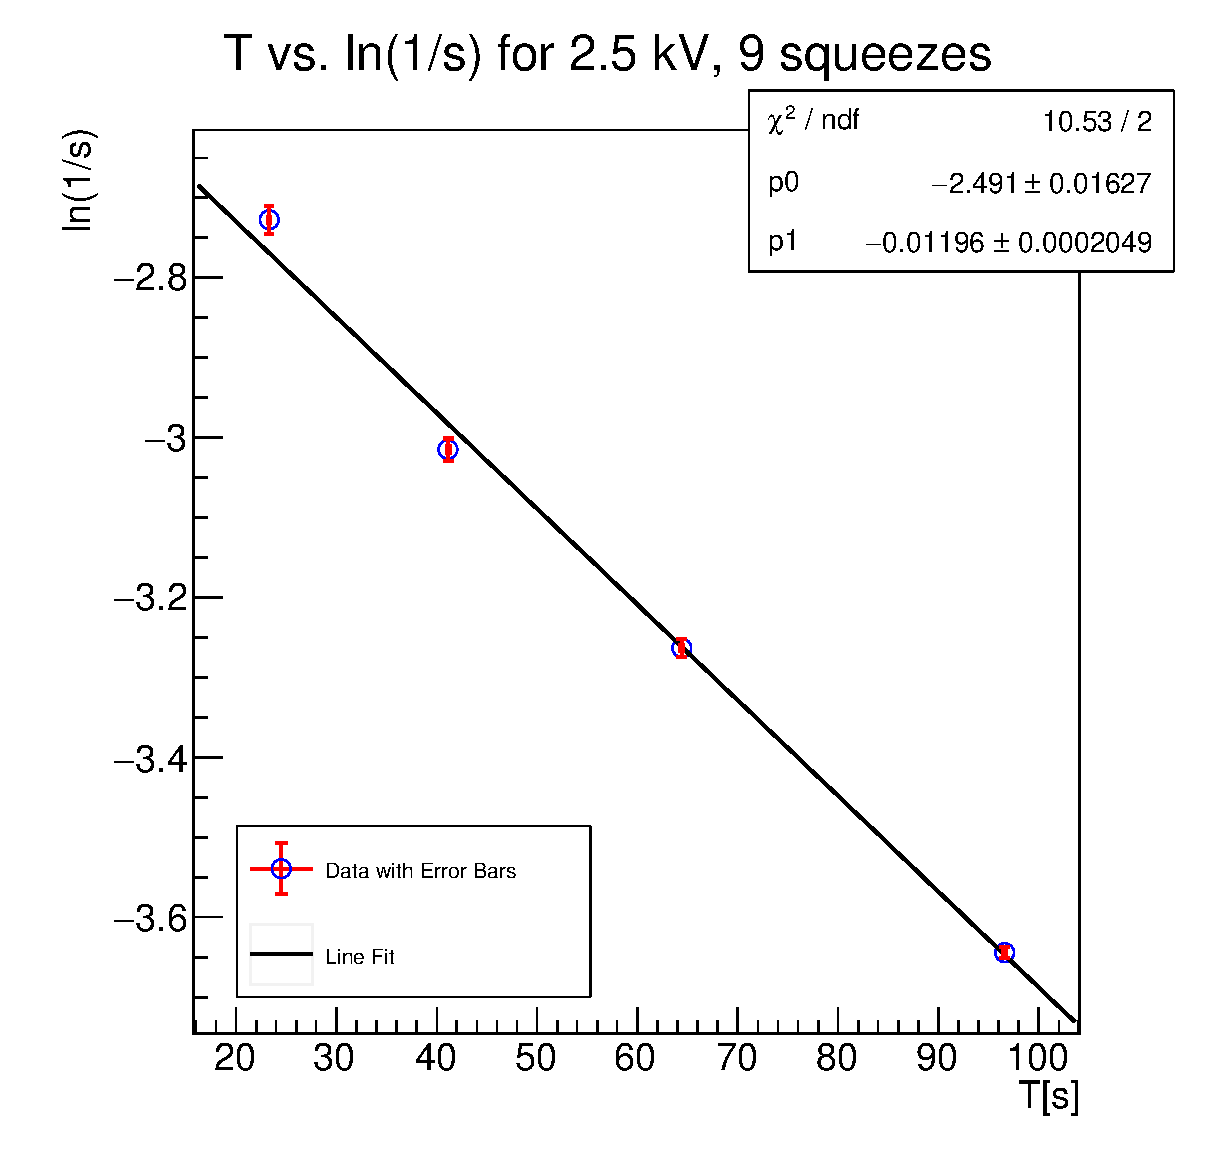
\includegraphics[width=0.95\columnwidth]{graphics/25_9.eps}
  \caption{Line regression for 2.5 kV and 9 squeezes. At each data point, error bars are drawn, where p0 is the y-intercept and p1 is the slope.}
\end{figure}




\begin{figure}[H]
  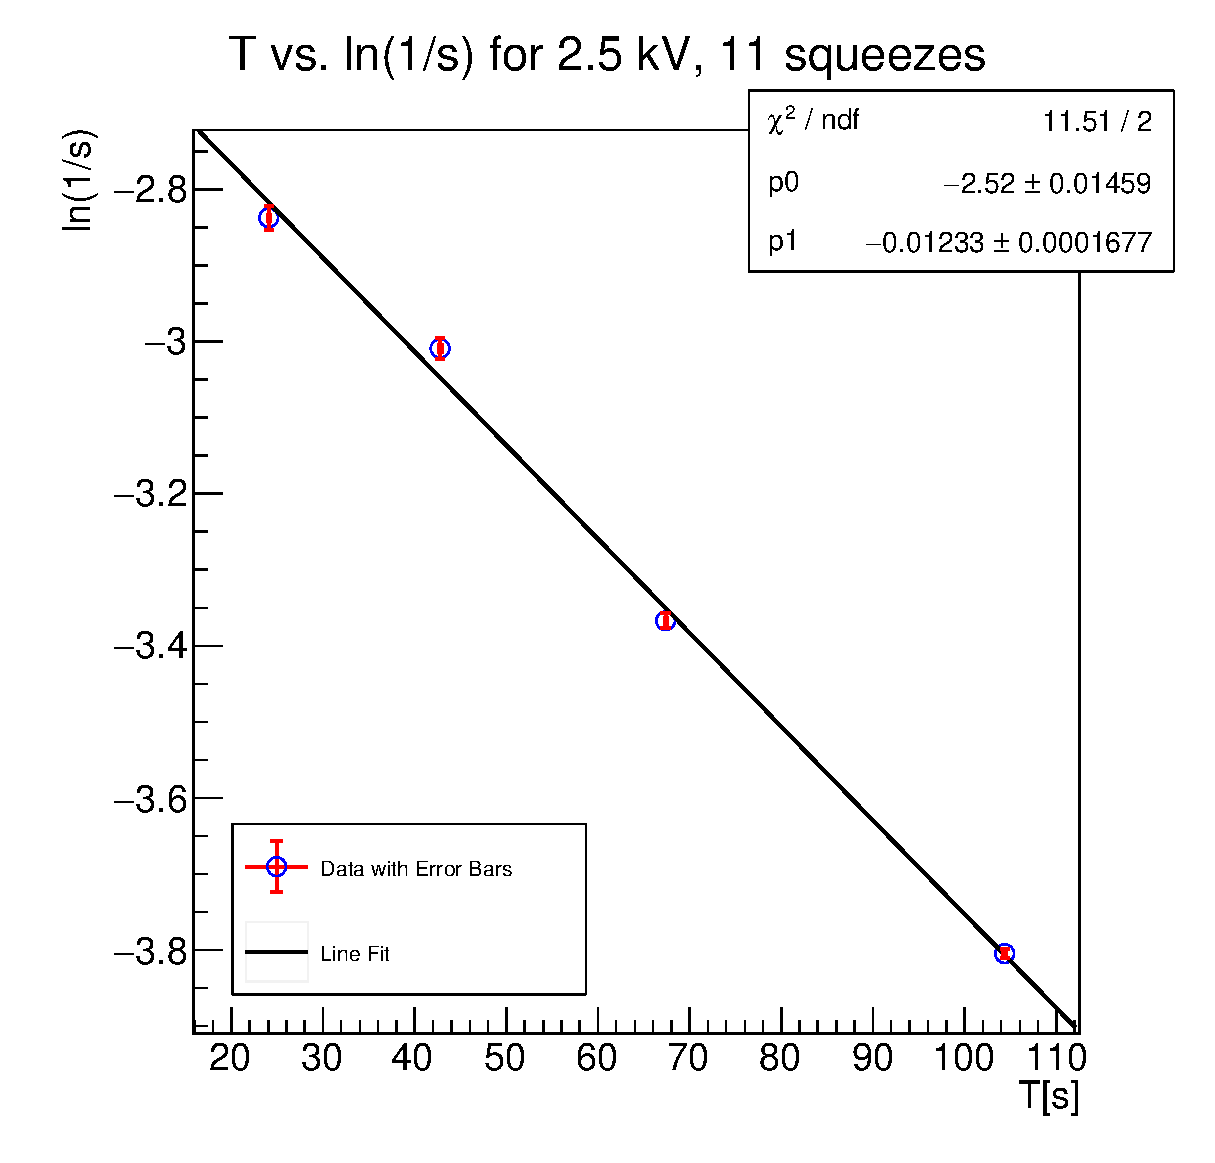
\includegraphics[width=0.95\columnwidth]{graphics/25_11.eps}
  \caption{Line regression for 2.5 kV and 11 squeezes. At each data point, error bars are drawn, where p0 is the y-intercept and p1 is the slope.}
\end{figure}


\subsection*{3.0 kV}

\begin{table}[H]
\caption{\label{tab:k}%
Calculations for $3000\si{\volt}$ with 5 squeezes.
}
\begin{ruledtabular}
\begin{tabular}{cccc}
\textrm{T[\si{\second}]}&
\textrm{$ln\left(\frac{1}{s}\right)$} &
\textrm{$\sigma_T$[\si{\second}]} &
\textrm{$\sigma_{ln\left(\frac{1}{s}\right)}$} \\ 
\colrule  
22.63  & -2.821 &  0.14   &  0.017 \\  
43.78  & -3.239 &  0.14   &  0.011 \\
75.37  & -3.629 &  0.14   &  0.008 \\
129.86 & -4.267 &  0.14   &  0.004
\end{tabular}  
\end{ruledtabular}
\end{table}

\begin{table}[H]
\caption{\label{tab:k}%
Calculations for $3000\si{\volt}$ with 7 squeezes.
}
\begin{ruledtabular}
\begin{tabular}{cccc}
\textrm{T[\si{\second}]}&
\textrm{$ln\left(\frac{1}{s}\right)$} &
\textrm{$\sigma_T$[\si{\second}]} &
\textrm{$\sigma_{ln\left(\frac{1}{s}\right)}$} \\ 
\colrule  
23.99  & -2.838 &  0.14  &   0.016 \\  
42.95  & -3.036 &  0.14  &   0.014 \\
66.74  & -3.287 &  0.14  &   0.010 \\
101.67 & -3.764 &  0.14  &   0.006
\end{tabular}  
\end{ruledtabular}
\end{table}

\begin{table}[H]
\caption{\label{tab:k}%
Calculations for $3000\si{\volt}$ with 9 squeezes.
}
\begin{ruledtabular}
\begin{tabular}{cccc}
\textrm{T[\si{\second}]}&
\textrm{$ln\left(\frac{1}{s}\right)$} &
\textrm{$\sigma_T$[\si{\second}]} &
\textrm{$\sigma_{ln\left(\frac{1}{s}\right)}$} \\ 
\colrule  
26.15 &  -2.842 &  0.14  &   0.016 \\   
45.56 &  -3.075 &  0.14  &   0.013 \\
71.60 &  -3.415 &  0.14  &   0.009 \\
111.26 & -3.890 &  0.14  &   0.006
\end{tabular}  
\end{ruledtabular}
\end{table}

\begin{table}[H]
\caption{\label{tab:k}%
Calculations for $3000\si{\volt}$ with 11 squeezes.
}
\begin{ruledtabular}
\begin{tabular}{cccc}
\textrm{T[\si{\second}]}&
\textrm{$ln\left(\frac{1}{s}\right)$} &
\textrm{$\sigma_T$[\si{\second}]} &
\textrm{$\sigma_{ln\left(\frac{1}{s}\right)}$} \\ 
\colrule  
18.64 &  -2.768 &  0.14  &   0.018   \\
36.33 &  -2.968 &  0.14  &   0.014   \\
59.50 &  -3.291 &  0.14  &   0.010   \\
92.23 &  -3.653 &  0.14  &   0.007
\end{tabular}  
\end{ruledtabular}
\end{table}

\begin{figure}[H]
  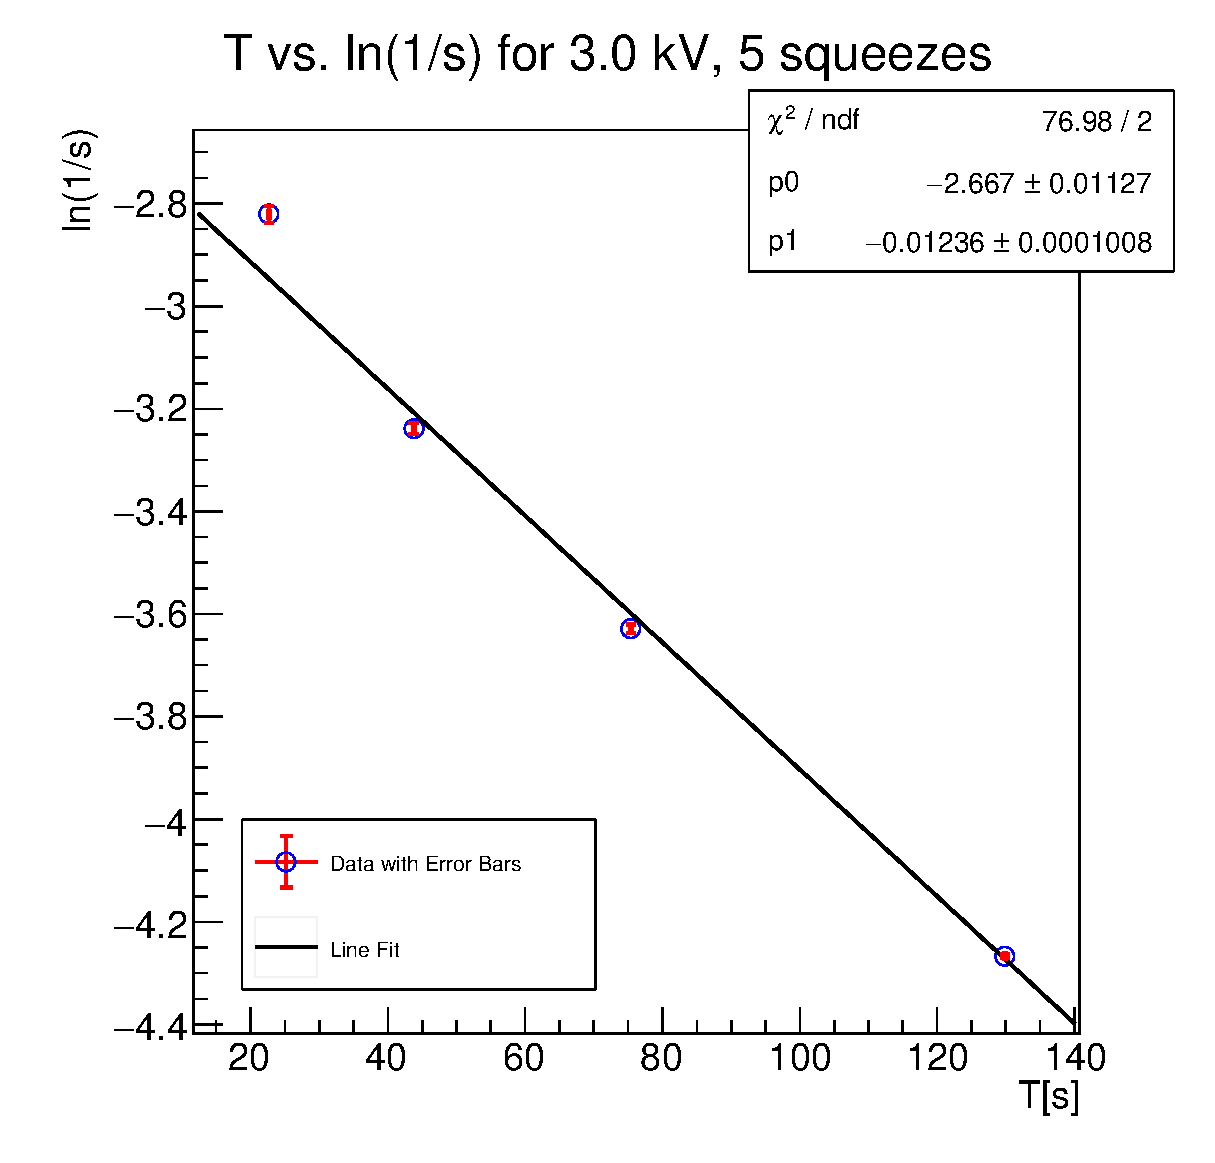
\includegraphics[width=0.95\columnwidth]{graphics/30_5.eps}
  \caption{Line regression for 3.0 kV and 5 squeezes. At each data point, error bars are drawn, where p0 is the y-intercept and p1 is the slope.}
\end{figure}




\begin{figure}[H]
  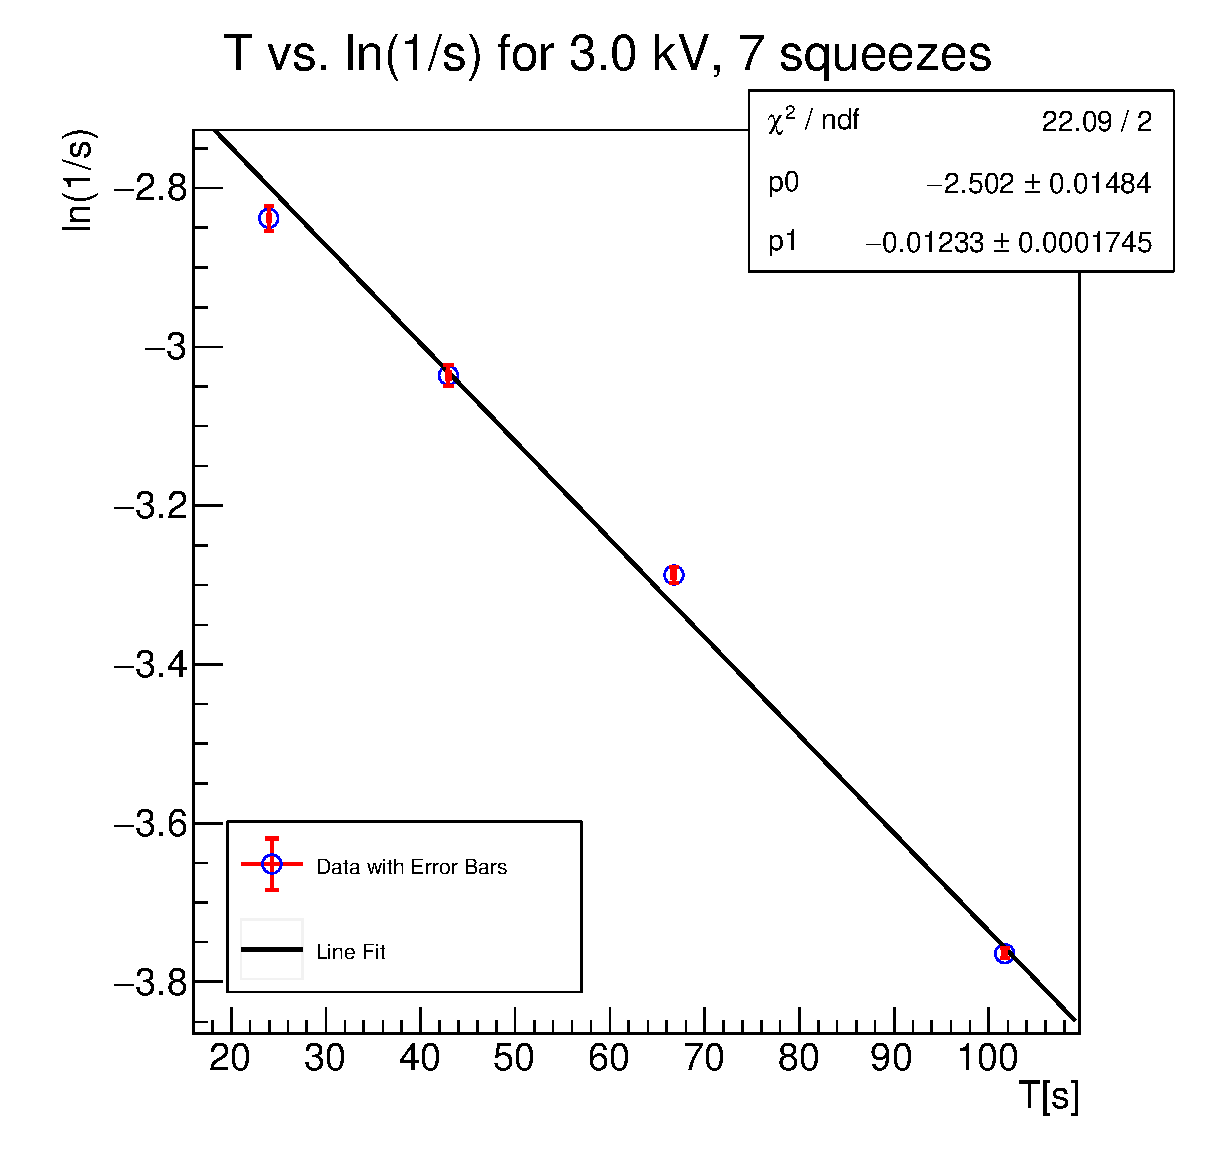
\includegraphics[width=0.95\columnwidth]{graphics/30_7.eps}
  \caption{Line regression for 3.0 kV and 7 squeezes. At each data point, error bars are drawn, where p0 is the y-intercept and p1 is the slope.}
\end{figure}




\begin{figure}[H]
  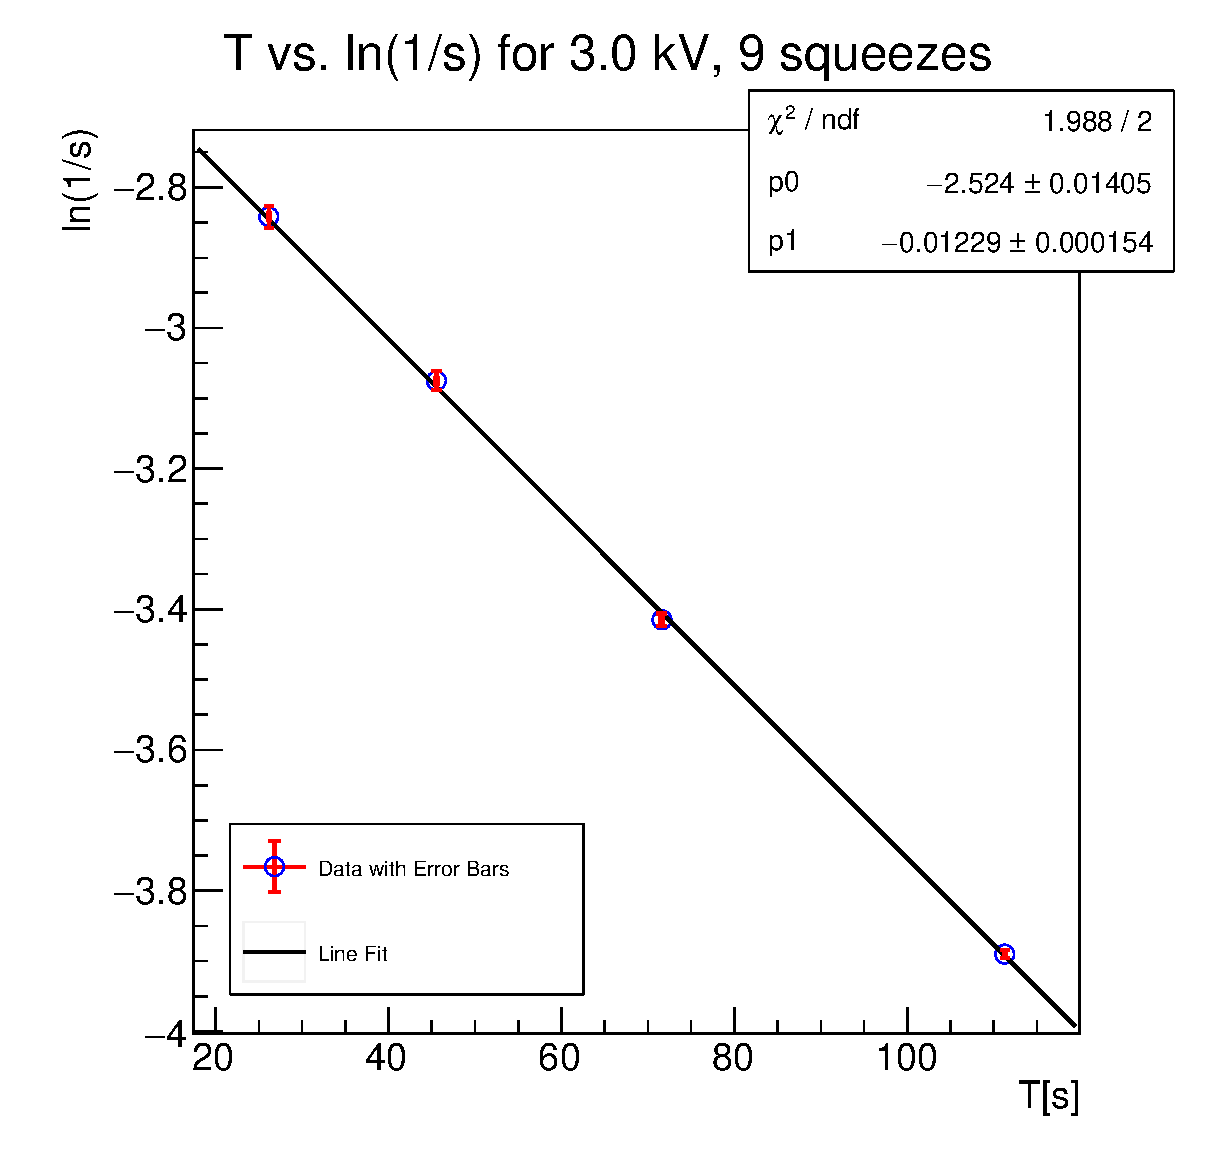
\includegraphics[width=0.95\columnwidth]{graphics/30_9.eps}
  \caption{Line regression for 3.0 kV and 9 squeezes. At each data point, error bars are drawn, where p0 is the y-intercept and p1 is the slope.}
\end{figure}





\begin{figure}[H]
  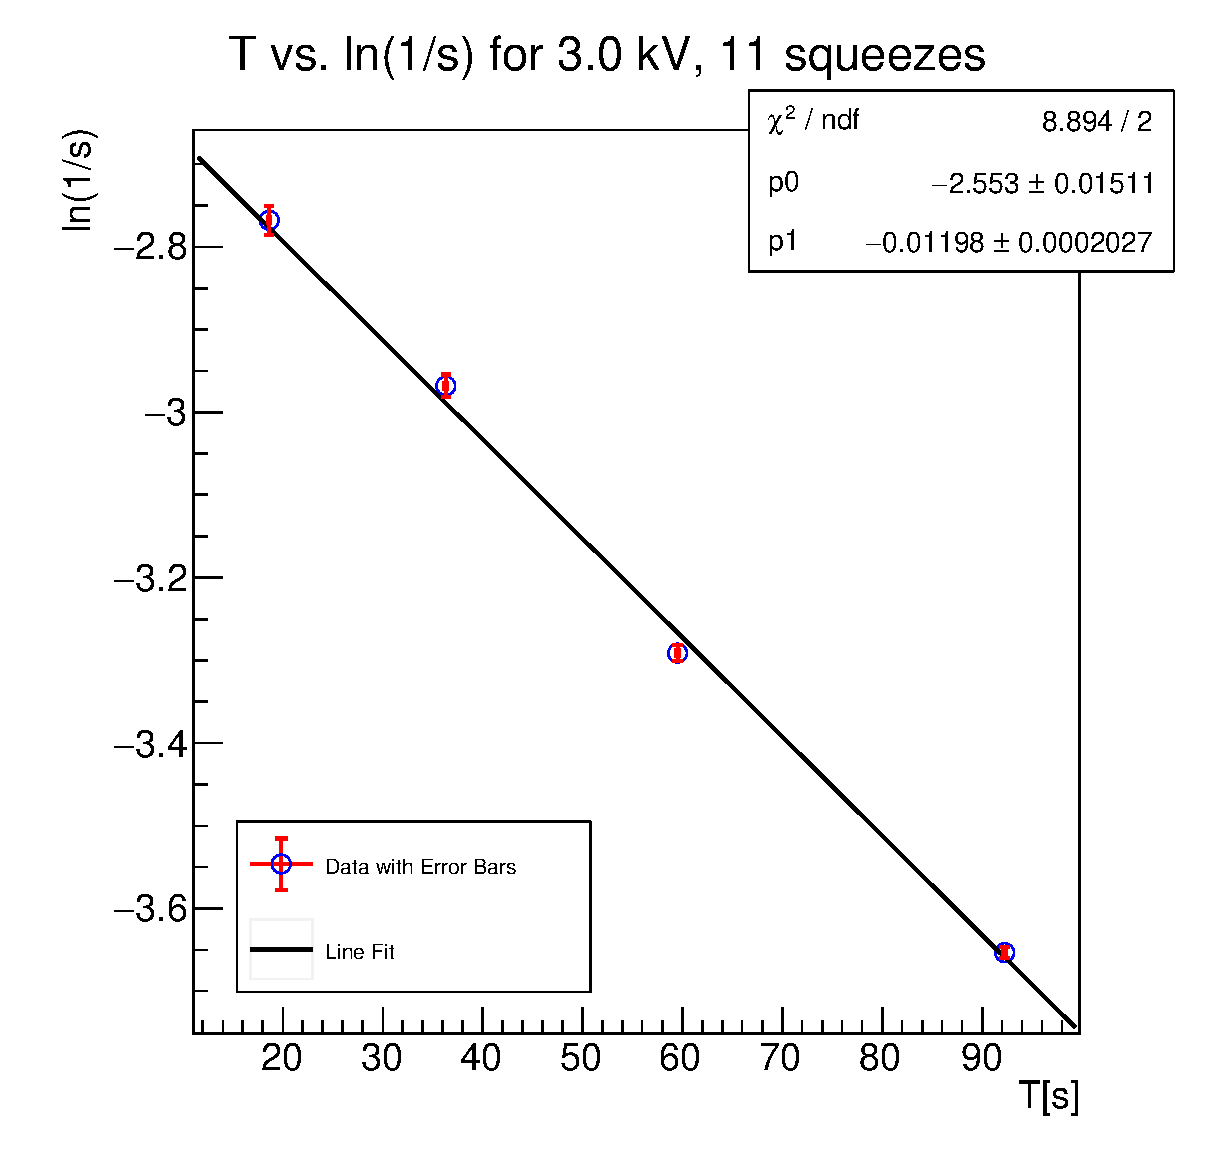
\includegraphics[width=0.95\columnwidth]{graphics/30_11.eps}
  \caption{Line regression for 3.0 kV and 11 squeezes. At each data point, error bars are drawn, where p0 is the y-intercept and p1 is the slope.}
\end{figure}

\subsection*{3.5 kV}

\begin{table}[H]
\caption{\label{tab:k}%
Calculations for $3500\si{\volt}$ with 5 squeezes.
}
\begin{ruledtabular}
\begin{tabular}{cccc}
\textrm{T[\si{\second}]}&
\textrm{$ln\left(\frac{1}{s}\right)$} &
\textrm{$\sigma_T$[\si{\second}]} &
\textrm{$\sigma_{ln\left(\frac{1}{s}\right)}$} \\ 
\colrule  
30.00 &  -3.006 &  0.14  &   0.014 \\   
53.42 &  -3.282 &  0.14  &   0.011 \\
87.91  & -3.746 &  0.14  &   0.007 \\
147.74 & -4.348 &  0.14  &   0.004
\end{tabular}  
\end{ruledtabular}
\end{table}

\begin{table}[H]
\caption{\label{tab:k}%
Calculations for $3500\si{\volt}$ with 7 squeezes.
}
\begin{ruledtabular}
\begin{tabular}{cccc}
\textrm{T[\si{\second}]}&
\textrm{$ln\left(\frac{1}{s}\right)$} &
\textrm{$\sigma_T$[\si{\second}]} &
\textrm{$\sigma_{ln\left(\frac{1}{s}\right)}$} \\ 
\colrule  
33.40  & -3.085 &  0.14  &   0.013 \\   
57.92  & -3.301 &  0.14  &   0.010 \\
93.57  & -3.788 &  0.14  &   0.006 \\
168.94 & -4.669 &  0.14  &   0.003
\end{tabular}  
\end{ruledtabular}
\end{table}

\begin{table}[H]
\caption{\label{tab:k}%
Calculations for $3500\si{\volt}$ with 9 squeezes.
}
\begin{ruledtabular}
\begin{tabular}{cccc}
\textrm{T[\si{\second}]}&
\textrm{$ln\left(\frac{1}{s}\right)$} &
\textrm{$\sigma_T$[\si{\second}]} &
\textrm{$\sigma_{ln\left(\frac{1}{s}\right)}$} \\ 
\colrule  
11.99 &  -2.684 &  0.14  &   0.019 \\  
27.98 &  -2.852 &  0.14  &   0.016 \\
47.67 &  -3.093 &  0.14  &   0.013 \\
74.58 &  -3.459 &  0.14  &   0.009
\end{tabular}  
\end{ruledtabular}
\end{table}

\begin{table}[H]
\caption{\label{tab:k}%
Calculations for $3500\si{\volt}$ with 11 squeezes.
}
\begin{ruledtabular}
\begin{tabular}{cccc}
\textrm{T[\si{\second}]}&
\textrm{$ln\left(\frac{1}{s}\right)$} &
\textrm{$\sigma_T$[\si{\second}]} &
\textrm{$\sigma_{ln\left(\frac{1}{s}\right)}$} \\ 
\colrule  
31.23 &  -2.968 &  0.14  &   0.014 \\   
53.92 &  -3.255 &  0.14  &   0.011 \\
86.29 &  -3.659 &  0.14  &   0.007 \\
145.08 & -4.366 &  0.14  &   0.004
\end{tabular}  
\end{ruledtabular}
\end{table}


\begin{figure}[H]
  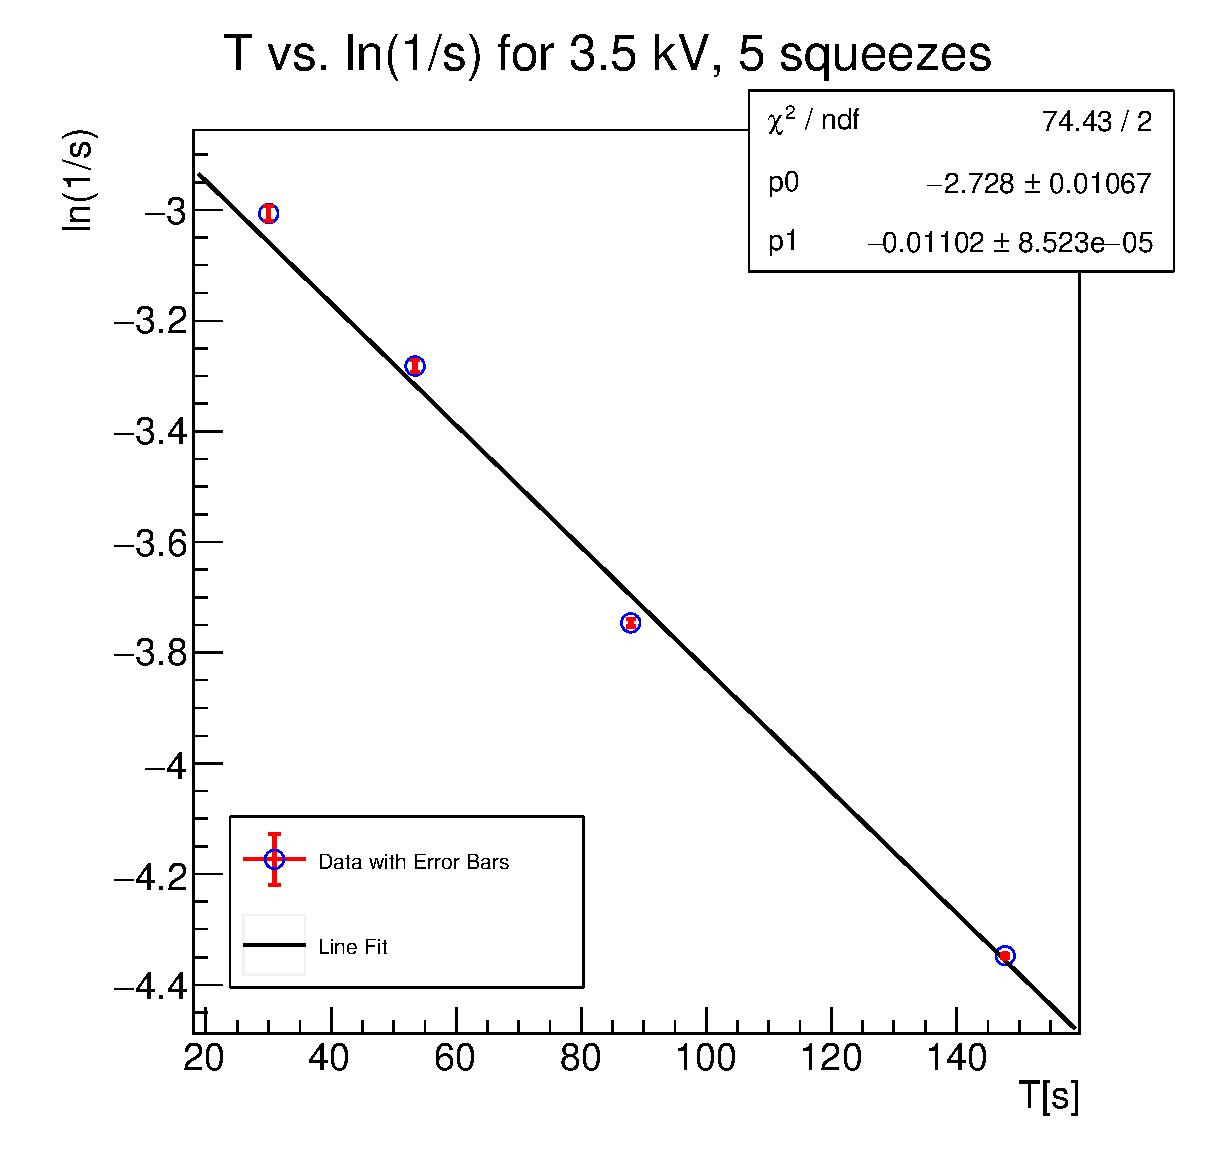
\includegraphics[width=0.95\columnwidth]{graphics/35_5.eps}
  \caption{Line regression for 3.5 kV and 5 squeezes. At each data point, error bars are drawn, where p0 is the y-intercept and p1 is the slope.}
\end{figure}




\begin{figure}[H]
  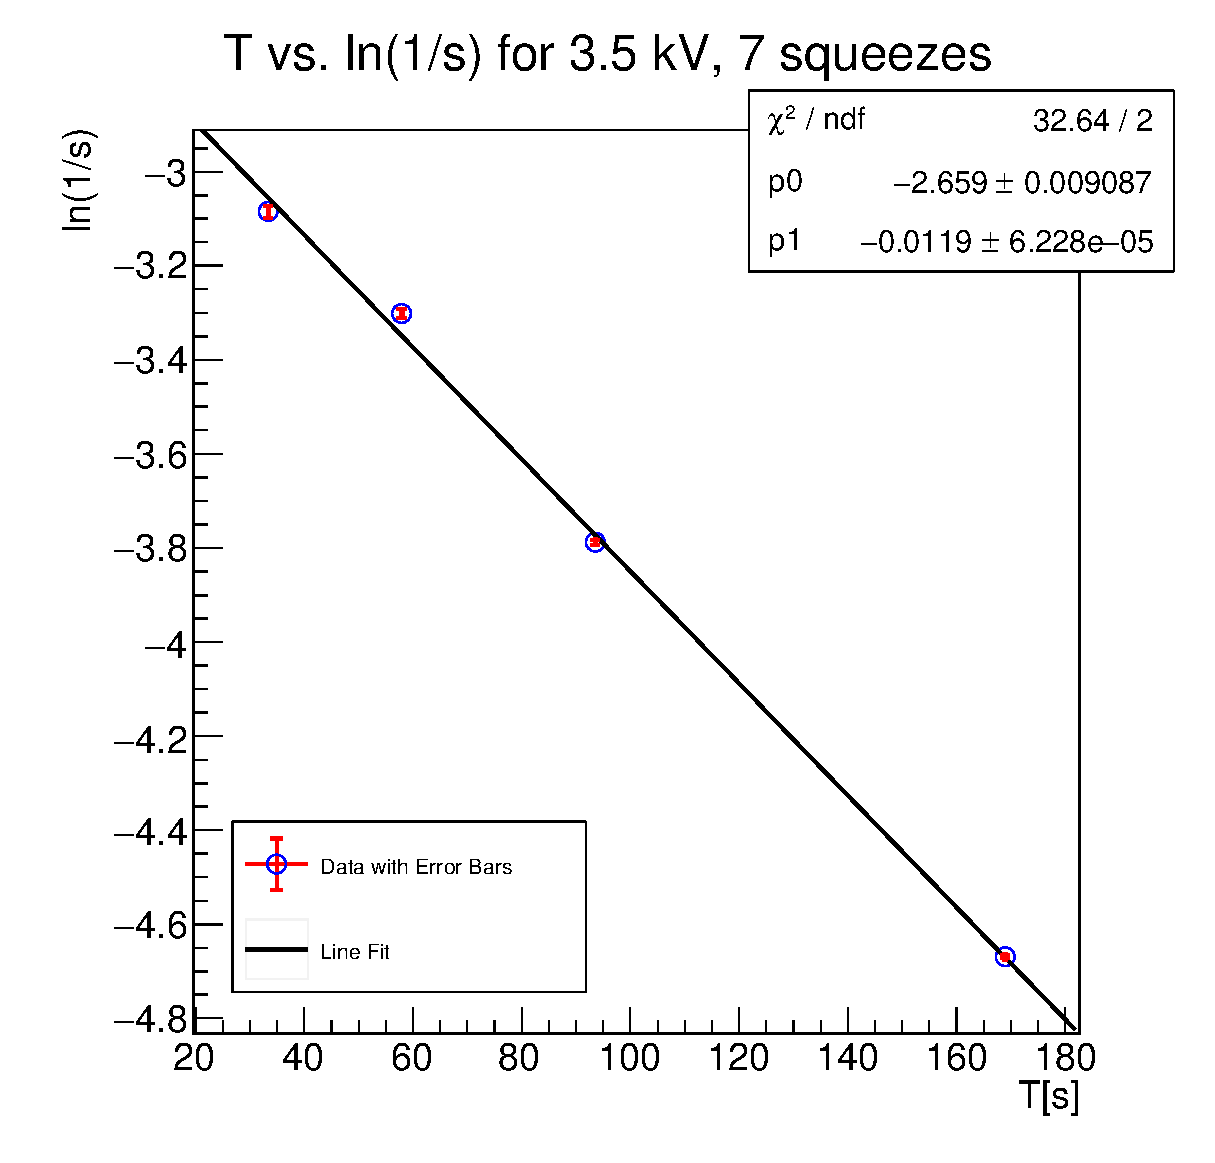
\includegraphics[width=0.95\columnwidth]{graphics/35_7.eps}
  \caption{Line regression for 3.5 kV and 7 squeezes. At each data point, error bars are drawn, where p0 is the y-intercept and p1 is the slope.}
\end{figure}




\begin{figure}[H]
  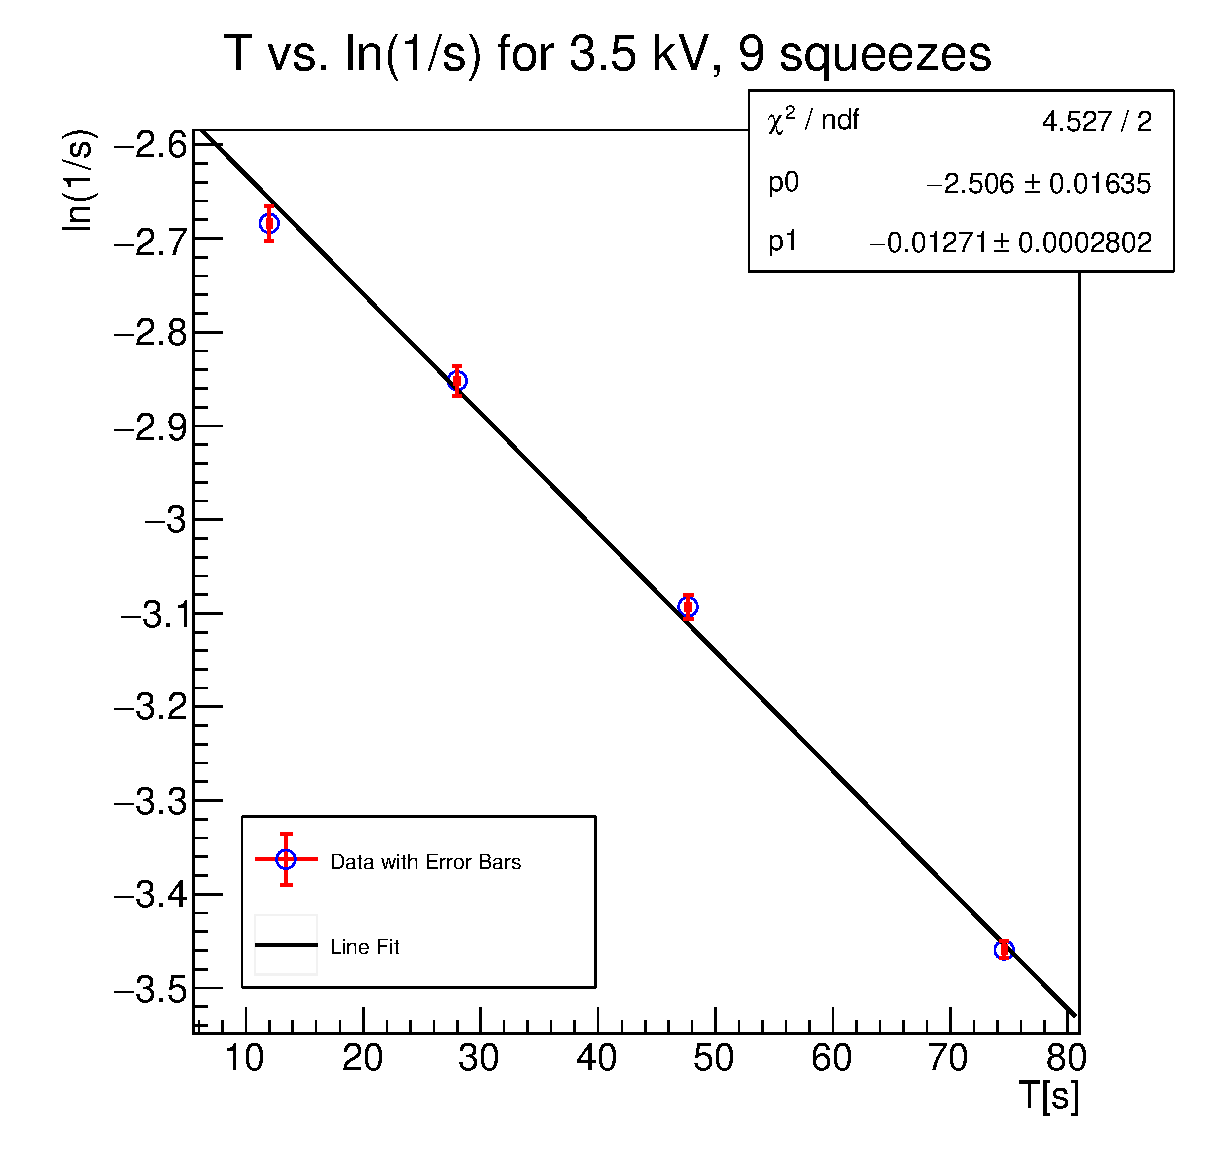
\includegraphics[width=0.95\columnwidth]{graphics/35_9.eps}
  \caption{Line regression for 3.5 kV and 9 squeezes. At each data point, error bars are drawn, where p0 is the y-intercept and p1 is the slope.}
\end{figure}




\begin{figure}[H]
  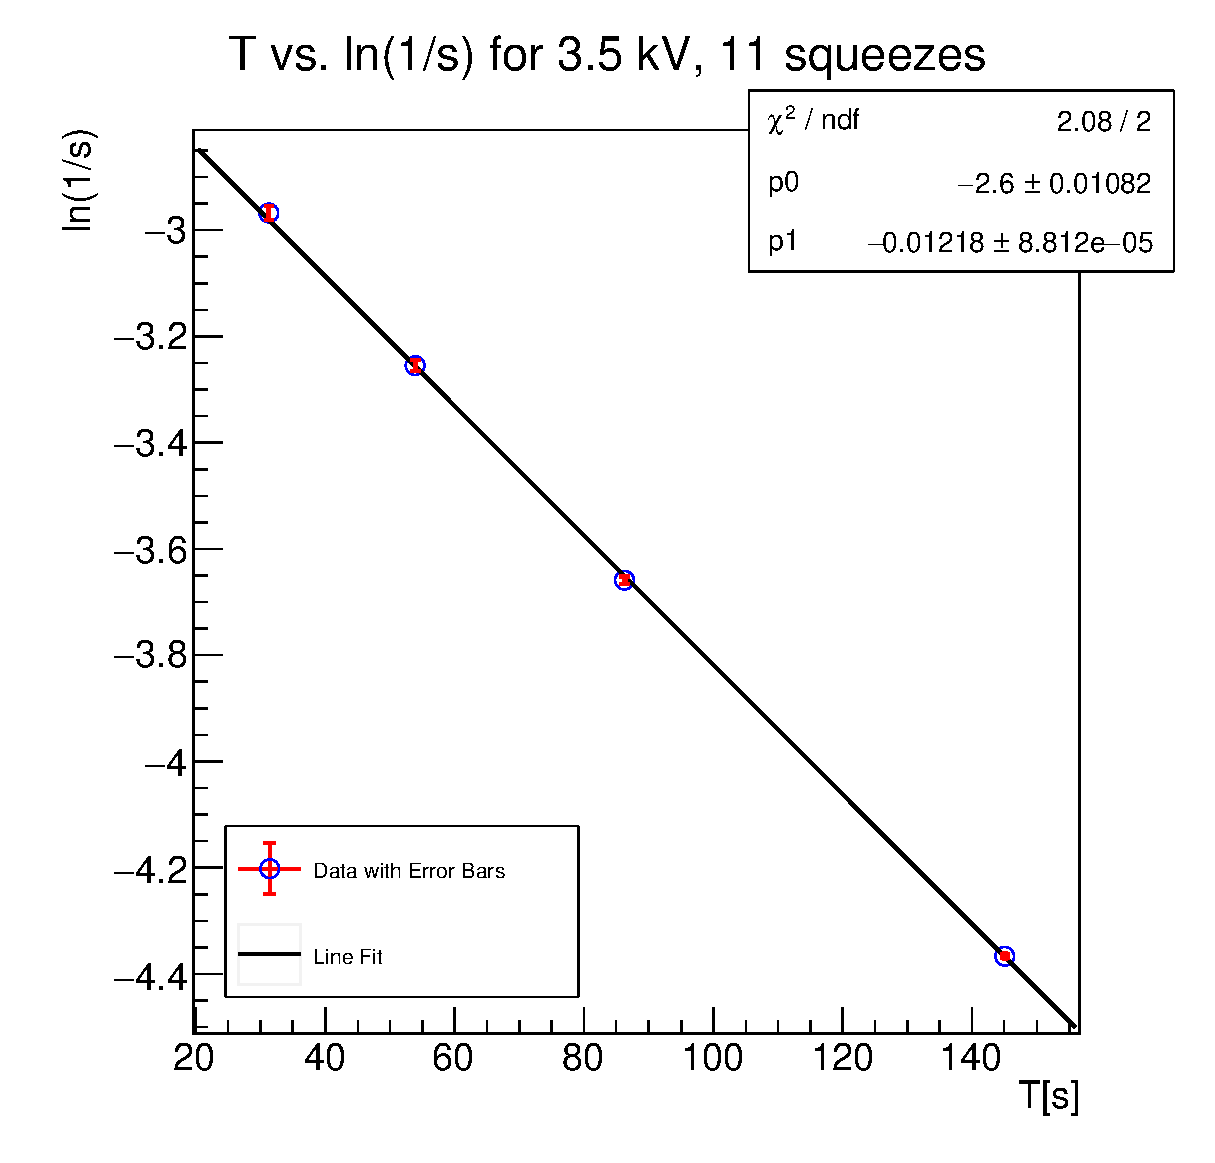
\includegraphics[width=0.95\columnwidth]{graphics/35_11.eps}
  \caption{Line regression for 3.5 kV and 11 squeezes. At each data point, error bars are drawn, where p0 is the y-intercept and p1 is the slope.}
\end{figure}
\newpage
Finally we can list our decay constants:
\begin{table}[H]
\caption{\label{tab:dc}%
Linear regressions for all data-sets. -slope is $\lambda$ with error $\sigma_\lambda$ and $\chi_\nu^2$ per degree of freedom $\nu$ is given.
}
\begin{ruledtabular}
\begin{tabular}{ccccc}
\textrm{Voltage$[\si{\kilo\volt}]$}&
\textrm{Squeezes}&
\textrm{$\lambda[s^{-1}]$}&
\textrm{$\sigma_\lambda[s^{-1}]$} &
\textrm{$\chi_\nu^2$} \\
\colrule  
2.5 & 5 & 0.01159 & 0.00010 & 1.536 \\
2.5 & 7 & 0.01457 & 0.00022 & 9.595 \\
2.5 & 9 & 0.01196 & 0.00020 & 2.632 \\
2.5 & 11 & 0.01233 & 0.00017 & 2.852 \\
\hline 
3.0 & 5 & 0.01236 & 0.00010 & 19.24 \\
3.0 & 7 & 0.01233 & 0.00017 & 5.522 \\
3.0 & 9 & 0.01229 & 0.00015 & 0.497 \\
3.0 & 11 & 0.01198 & 0.00020 & 2.224 \\
\hline 
3.5 & 5 & 0.01102 & 0.00008 & 18.61 \\
3.5 & 7 & 0.01190 & 0.00006 & 8.160 \\
3.5 & 9 & 0.01271 & 0.00028 & 1.132 \\
3.5 & 11 & 0.01218 & 0.00009 & 0.520 
\end{tabular}  
\end{ruledtabular}
\end{table}

Observe that number of squeezes and applied voltage does not affect the slopes. \\

Let's calculate weighted average of slopes and it's error with using \eqref{eq:mean} and \eqref{eq:meanstd}. We get:

\begin{align}
  \lambda_\mu = (0.01193 \pm 0.00003) s^{-1}
\end{align} 

With using \eqref{eq:half} we can calculate the half-time of the Radon gas($^{220}Rn$) with error propagation \eqref{eq:err}:

\begin{align}
    t_{1/2} &= \frac{ln(2)}{\lambda_\mu} = (58.10 \pm 0.15) s 
\end{align}


\section{Conclusion and Possible Error Sources}
The accepted half-time for $^{220}Rn$ is given $55.6 s$. Our result is $ t_{1/2} =(58.1 \pm 0.2) s $ and it has very low relative uncertainty about $0.34 \%$. This makes our result  $12 \sigma$'s away from accepted value and it is too much. The reason for this can be the selection of average human response time since it is mainly determines the uncertianty of the measurements in our experiment and may be our response time wasn't that great at all. If we look our percentage error is $4.68\%$, which is not that bad.\\

The possible error sources can be listed:

\begin{itemize}
  \item We assumed the last product in the decay is $^{220}Rn$. However, if we look at the chain reaction there are other products are may be formed and this can affect our results.\cite{conc}
  \item We may not have emptied the ionization chamber correctly this can be problem if there are radioactive material left in the chamber.
\end{itemize}
\newpage
\appendix
\section{Measurements}

\subsection{2500 V}

\begin{table}[H]
\caption{\label{tab:kv25}%
Time measurements for $2500\si{\volt}$ with using different squeezes.
}
\begin{ruledtabular}
\begin{tabular}{ccccc}
\textrm{Squeezes :} &
\textrm{5} &
\textrm{7} &
\textrm{9} &
\textrm{11} \\ 
\colrule  
\textit{$t_1$}\hspace{1mm}[$\si{\second}]$& 13.03  & 7.09   & 15.64 & 15.57  \\
\textit{$t_2$}\hspace{1mm}[$\si{\second}]$& 32.11  & 20.67  & 30.94 & 32.64  \\
\textit{$t_3$}\hspace{1mm}[$\si{\second}]$& 57.92  & 40.41  & 51.33 & 52.91  \\
\textit{$t_4$}\hspace{1mm}[$\si{\second}]$& 94.91  & 65.26  & 77.47 & 81.89  \\
\textit{$t_5$}\hspace{1mm}[$\si{\second}]$& 161.89 & 106.87 & 115.70 & 126.82    
\end{tabular}  
\end{ruledtabular}
\end{table}


\subsection{3000 V}

\begin{table}[H]
\caption{\label{tab:kv30}%
Time measurements for $3000\si{\volt}$ with using different squeezes.
}
\begin{ruledtabular}
\begin{tabular}{ccccc}
\textrm{Squeezes :} &
\textrm{5} &
\textrm{7} &
\textrm{9} &
\textrm{11} \\ 
\colrule  
\textit{$t_1$}\hspace{1mm}[$\si{\second}]$&14.23     & 15.45      & 17.57  & 10.68  \\
\textit{$t_2$}\hspace{1mm}[$\si{\second}]$&31.03     & 32.53      & 34.73  & 26.60  \\
\textit{$t_3$}\hspace{1mm}[$\si{\second}]$&56.53     & 53.36      & 56.39  & 46.06  \\
\textit{$t_4$}\hspace{1mm}[$\si{\second}]$&94.20     & 80.12      & 86.80  & 72.94  \\
\textit{$t_5$}\hspace{1mm}[$\si{\second}]$&165.53    & 123.22     & 135.72 & 111.52 
\end{tabular}  
\end{ruledtabular}
\end{table}

\subsection{3500 V}

\begin{table}[H]
\caption{\label{tab:kv35}%
Time measurements for $3500\si{\volt}$ with using different squeezes.
}
\begin{ruledtabular}
\begin{tabular}{ccccc}
\textrm{Squeezes :} &
\textrm{5} &
\textrm{7} &
\textrm{9} &
\textrm{11} \\ 
\colrule  
\textit{$t_1$}\hspace{1mm}[$\si{\second}]$& 19.90     & 22.47      & 4.67   & 21.50 \\ 
\textit{$t_2$}\hspace{1mm}[$\si{\second}]$& 40.10     & 44.34      & 19.31  & 40.96 \\ 
\textit{$t_3$}\hspace{1mm}[$\si{\second}]$& 66.73     & 71.49      & 36.64  & 66.87 \\ 
\textit{$t_4$}\hspace{1mm}[$\si{\second}]$& 109.08    & 115.65     & 58.69  & 105.70 \\ 
\textit{$t_5$}\hspace{1mm}[$\si{\second}]$& 186.41    & 222.22     & 90.48  & 184.46
\end{tabular}  
\end{ruledtabular}
\end{table}



\section{Mathematical Concepts}

\subsection{Chi-squared Test}
$\chi^2$ can be defined as:
\begin{align}
  \chi^2_\nu = \sum \frac{(y_i -y(x_i))^2}{\sigma^2_i}
\end{align}
$\chi^2$ per degrees of freedom:
\begin{align}
  \chi^2_\nu = \frac{1}{\nu} \sum \frac{(y_i -y(x_i))^2}{\sigma^2_i}
\end{align}
where $\nu$ is the number of degrees of freedom; the number of data points minus the number of parameters: $N-m$.

\subsection{Least Squares Method}

Let's define line for fitting as $y_i = a_0 + a_1x_i$
Parameters are
\begin{align}
  a_0 &= \frac{1}{D}\left(\sum_{k}^{N}\frac{x^2_k}{\sigma^2_k} \sum_{k}^{N}\frac{y_k}{\sigma^2_k} - \sum_{k}^{N}\frac{x_k}{\sigma^2_k} \sum_{k}^{N}\frac{x_k y_k}{\sigma^2_k}\right) \\
    a_1 &= \frac{1}{D}\left(\sum_{k}^{N}\frac{1}{\sigma^2_k} \sum_{k}^{N}\frac{x_k y_k}{\sigma^2_k} - \sum_{k}^{N}\frac{x_k}{\sigma^2_k} \sum_{k}^{N}\frac{y_k}{\sigma^2_k}\right) \\
    D &= \sum_{k}^{N}\frac{1}{\sigma^2_k} \sum_{k}^{N}\frac{x^2_k}{\sigma^2_k} - \left(\sum_{k}^{N}\frac{x_k}{\sigma^2_k}\right)^2
\end{align}
Uncertainties of Parameters are:
\begin{align}
\sigma^2_{a_0} = \frac{1}{D} \sum_{k}^{N}\frac{x^2_j}{\sigma^2_j} \\
\sigma^2_{a_1} = \frac{1}{D} \sum_{k}^{N}\frac{1}{\sigma^2_j}
\end{align}

\subsection{Error Propagation}
\begin{align}
  \sigma^2_y = \sum_i^m \left(\frac{\partial f}{\partial x_i}\right)^2 \sigma^2_i \label{eq:err}
\end{align}

\subsection{Total Uncertainty}
\begin{align}
  \sigma^2 = \sigma_{systematic}^2 + \sigma_{instrumental}^2 + \sigma_{statistical}^2 \label{eq:unc}
\end{align}

\subsection{Weighted Mean and Standart Deviation} 
Mean:
\begin{align}
\mu = \frac{\sum\limits_i^N x_i / \sigma_i^2}{\sum\limits_i^N 1/\sigma_i^2} \label{eq:mean}
\end{align}
Standard Deviation:
\begin{align}
  \sigma^2 \simeq \frac{1}{\sum\limits_i^N 1/\sigma_i^2}  \label{eq:meanstd}
\end{align}


\newpage
\nocite{*}
\bibliography{report}

\end{document}
